\begin{table}[ht]       % provavelmente devo meter as palavras "parameter"/"base station" na caption?
	\centering          % ou devo eliminar a celula toda?
    \captionsetup{justification=centering}
    \caption{Compilation of the most relevant solutions available in the market (as of the date of the present document).}
	\label{tab:current_solutions_1}
	\begin{tabular}{|c|c|c|c|c|c|} % 8 colunas
		\toprule
		
        {} & {} & {} & \vtop{\hbox{\strut \textbf{beRTK}}\hbox{\strut \textbf{(Beyond Vision)}}} & \vtop{\hbox{\strut \textbf{Reach RS2}}\hbox{\strut \textbf{(Emlid)}}} & \vtop{\hbox{\strut \textbf{D-RTK 2}}\hbox{\strut \textbf{(DJI)}}}\\        
        
        \midrule

        \multirow{8}{*}{\rotatebox{90}{\textbf{Positioning}}}&\textbf{CorrectionT}\\
        &\multirow{5}{*}{\rotatebox{90}{\textbf{SupportedC}}}&\textbf{GPS}\\
        &\textbf{GLONASS}\\
        &X\\
        &X\\
        &X\\
        &X\\
        &X\\
        \midrule
        
        \rotatebox{90}{\textbf{Connectivity}} & 2 & 2 & 2 & 2 & 2\\
        \midrule

        \multirow{2}{*}{Multirow}&X\\
        &X & t\\

        \midrule\addlinespace[1.5ex]
        
        {} & 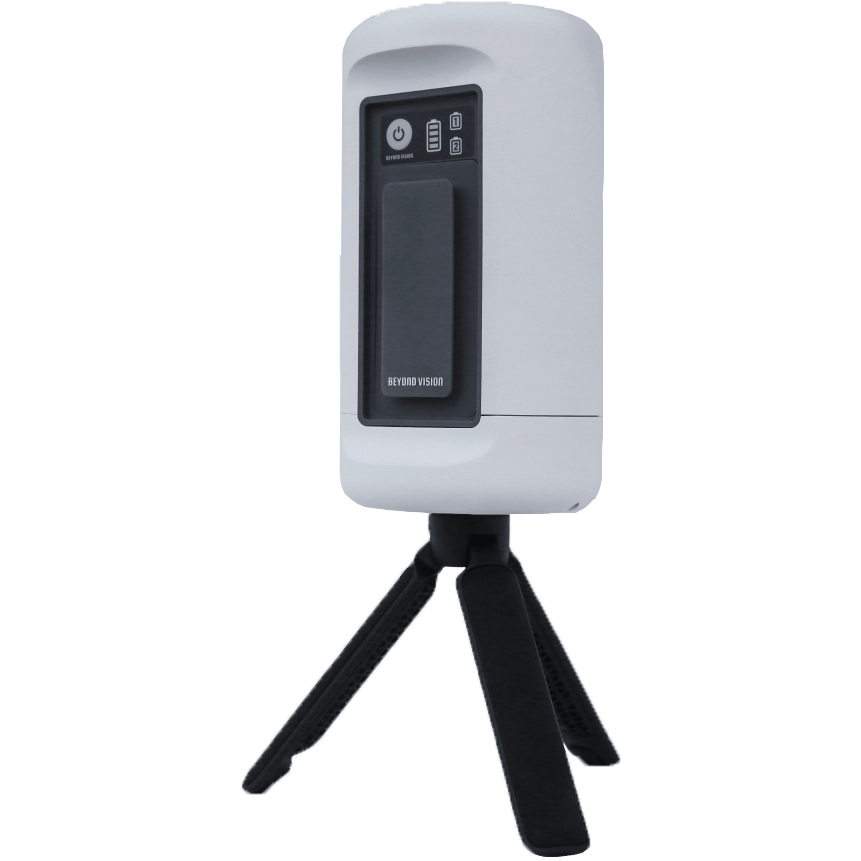
\includegraphics[height=1.4cm]{Chapters/Figures/base_stations/beRTK_2.png} & 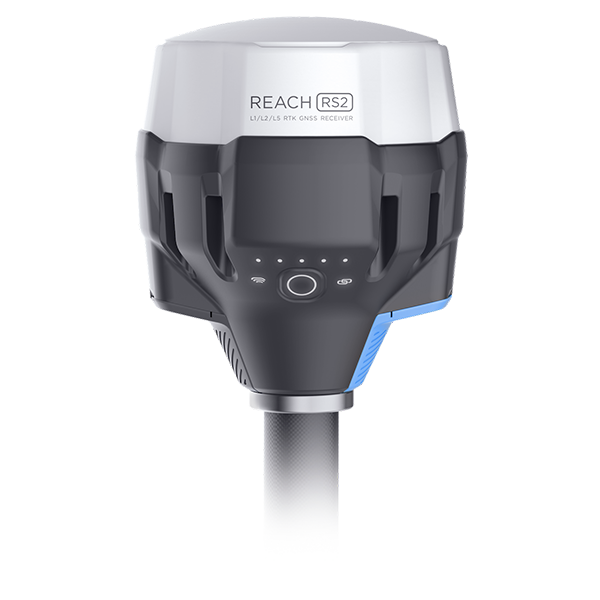
\includegraphics[height=1.4cm]{Chapters/Figures/base_stations/REACH-RS2.png} & 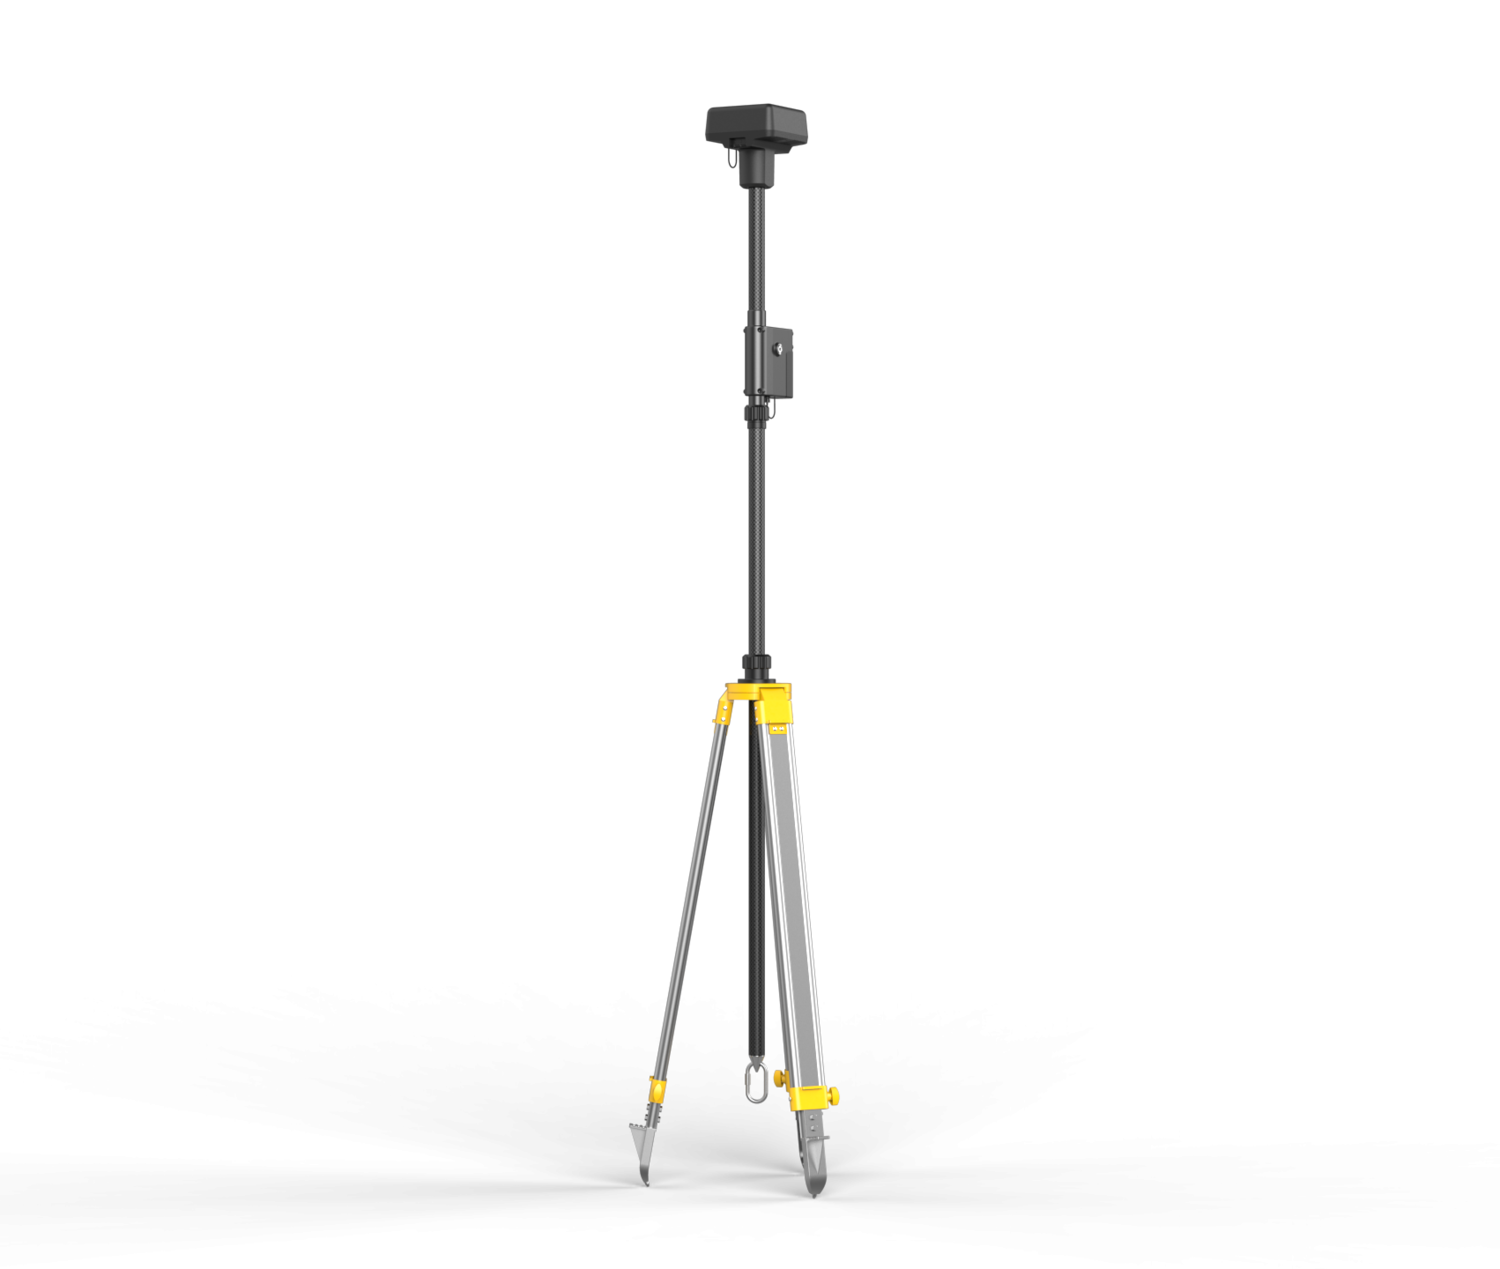
\includegraphics[height=1.4cm]{Chapters/Figures/base_stations/d-rtk-2.png}\\
		
        \bottomrule
        
	\end{tabular}
\end{table}

% tabela como multirow dento de multirow:
% \multirow{6}{*}{W2} & \multirow{3}{*}{3} & $0.090475\pm 0.011115$ & \multirow{3}{*}{21} & \multirow{3}{*}{6} & \multirow{3}{*}{3} \\
                    % &                    & $0.14861\pm 0.03562$   &                     &                    &                    \\
                    % &                    & $0.1861 \pm 0.01728$   &                     &                    &                    \\
                    % & 6                  & 8                      & 14                  & 5                  & 2                  \\
                    % & 9                  & 8                      & 14                  & 5                  & 2                  \\
                    % & 12                 & 8                      & 14                  & 5                  & 2                  \\


% \begin{table}[ht]
%     \centering
%     \captionsetup{justification=centering}
%     \caption{Compilation of the most relevant solutions available in the market (as of the date of the present document).}
% 	\label{tab:curr_solutions_positioning}
%     \begin{tabular}{cccccccc} % 8 colunas
% 		\toprule
%         \multicolumn{8}{c}{\textbf{Positioning}}\\
%         \textbf{CorrectionT} &.
% 		\multicolumn{5}{c}{\textbf{SupportedC}}\\
%         \textbf{GPS}&   \textbf{GLONASS}   &   \textbf{Galileo}   &   \textbf{BeiDou}   &   \textbf{NavIC}\\
%         \bottomrule
% 	\end{tabular}
% \end{table}


\begin{table}[ht]       % provavelmente devo meter as palavras "parameter"/"base station" na caption?
	\centering          % ou devo eliminar a celula toda?
    \captionsetup{justification=centering}
    \caption{Compilation of the most relevant solutions available in the market (as of the date of the present document).}
	\label{tab:current_solutions_2}
	\begin{tabular}{|c|c|c|c|c|} % 8 colunas
		\toprule
		{} & {} & {} & \vtop{\hbox{\strut \textbf{HiPer V}}\hbox{\strut \textbf{(Topcon)}}} & \vtop{\hbox{\strut \textbf{S990A GNSS Receiver}}\hbox{\strut \textbf{(Stonex)}}}\\        
        \midrule
        \rotatebox{90}{\textbf{pizza}} & 2 & 2 & 2 & 2\\
        \midrule\addlinespace[1.5ex]
        {} & 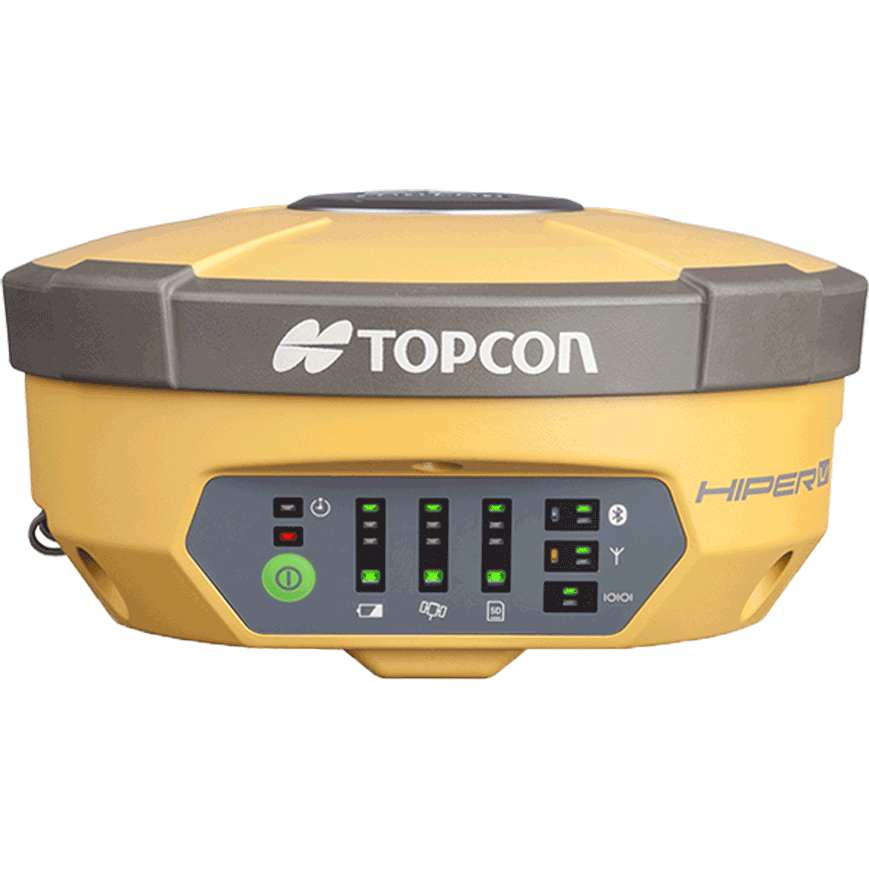
\includegraphics[height=1.4cm]{Chapters/Figures/base_stations/HiPer-V.png} & 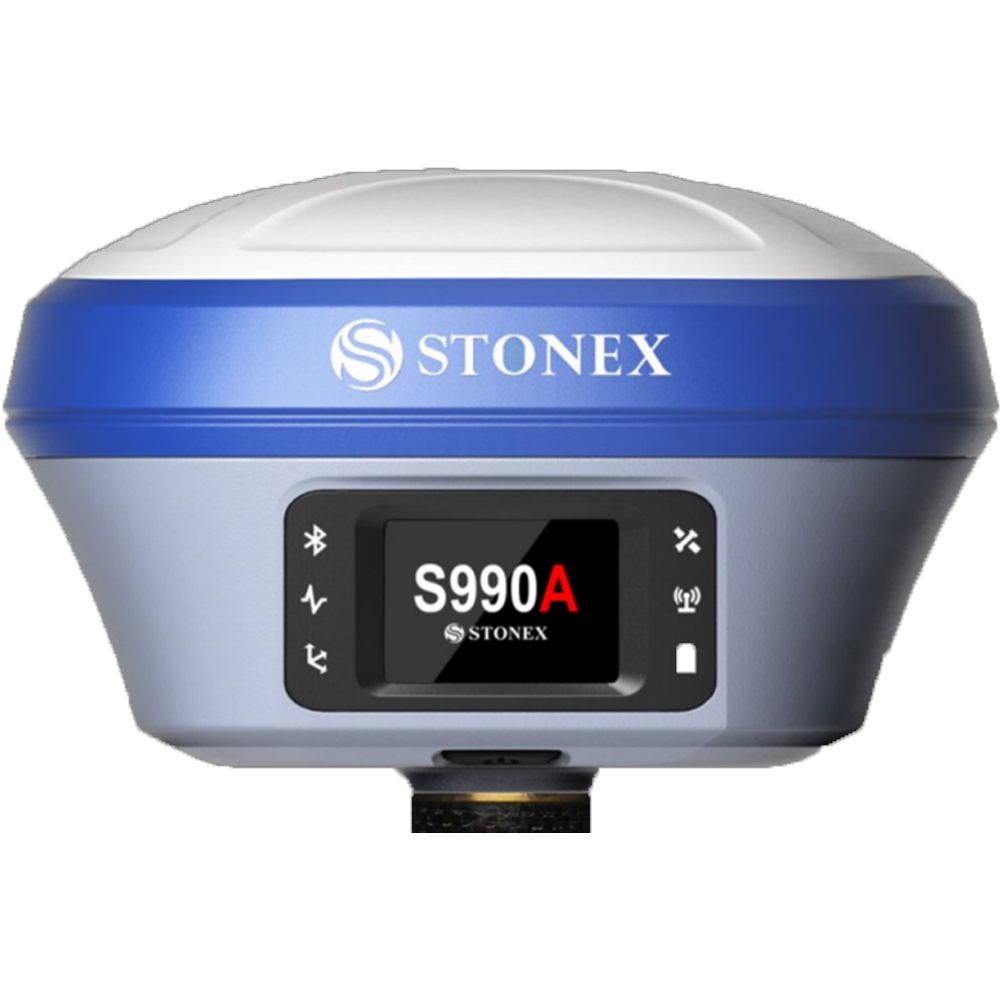
\includegraphics[height=1.4cm]{Chapters/Figures/base_stations/S990A.png}\\
		\bottomrule
	\end{tabular}
\end{table}


% tabela com palavras rodadas:
% \begin{tabular}{m{1em}c}
%     \rotatebox{90}{\textbf{Electrical }}& \makecell{\textbf{Supply} \\ \textbf{Input}\\ \textbf{Battery} \\ \textbf{Autonomy}}\\
% \end{tabular}\\

\newcolumntype{M}[1]{>{\centering\arraybackslash}m{#1}}
\begin{table}[ht]
    \centering
    \captionsetup{justification=centering}
    \caption{Compilation of the most relevant solutions available in the market (as of the date of the present document).}
	\label{tab:currednt_solutions}
    \begin{tabular}{|M{2.5cm}|M{2.5cm}|M{2.5cm}|}
      \hline
      Reconstruction strategy & aa          & bb( \%) \\ \hline
      Classic                 & 3342 voxels & 68 \%   \\ \hline
      VC                      & 4296 voxels & 87 \%   \\ \hline
      V m=7                   & 4745 voxels & 96 \%   \\ \hline
    \end{tabular}
\end{table}

\begin{table}[ht] 
    \centering 
    \begin{tabular}{  >{\raggedright}m{4.5cm}  m{5cm}}      % centered columns (3 columns) 
    \toprule                                   %inserts double horizontal lines 
    Building Block  & Circuits\\  % inserts table heading 
    \midrule\addlinespace[1.5ex]
            Inverting op-amp\\
            (linear amplifier)
            & 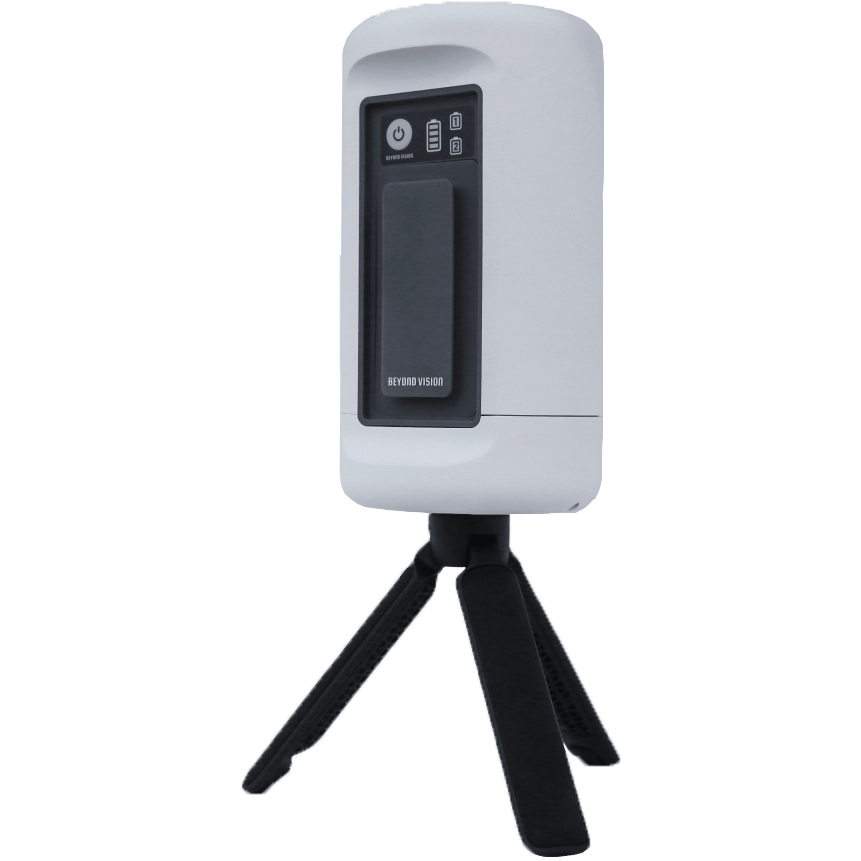
\includegraphics[height=1cm]{Chapters/Figures/base_stations/beRTK_2.png} \\
    \midrule\addlinespace[1.5ex]
            Integrator 
            & 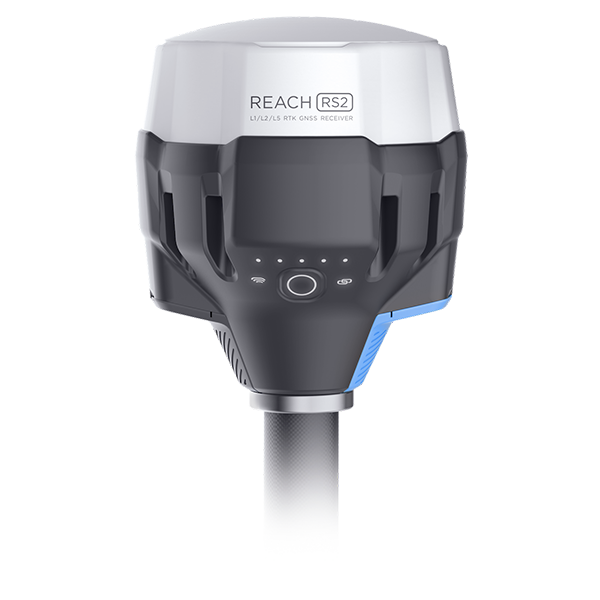
\includegraphics[height=1cm]{Chapters/Figures/base_stations/REACH-RS2.png} \\
    \midrule\addlinespace[1.5ex]
            AC integrator \\ with DC gain
            & 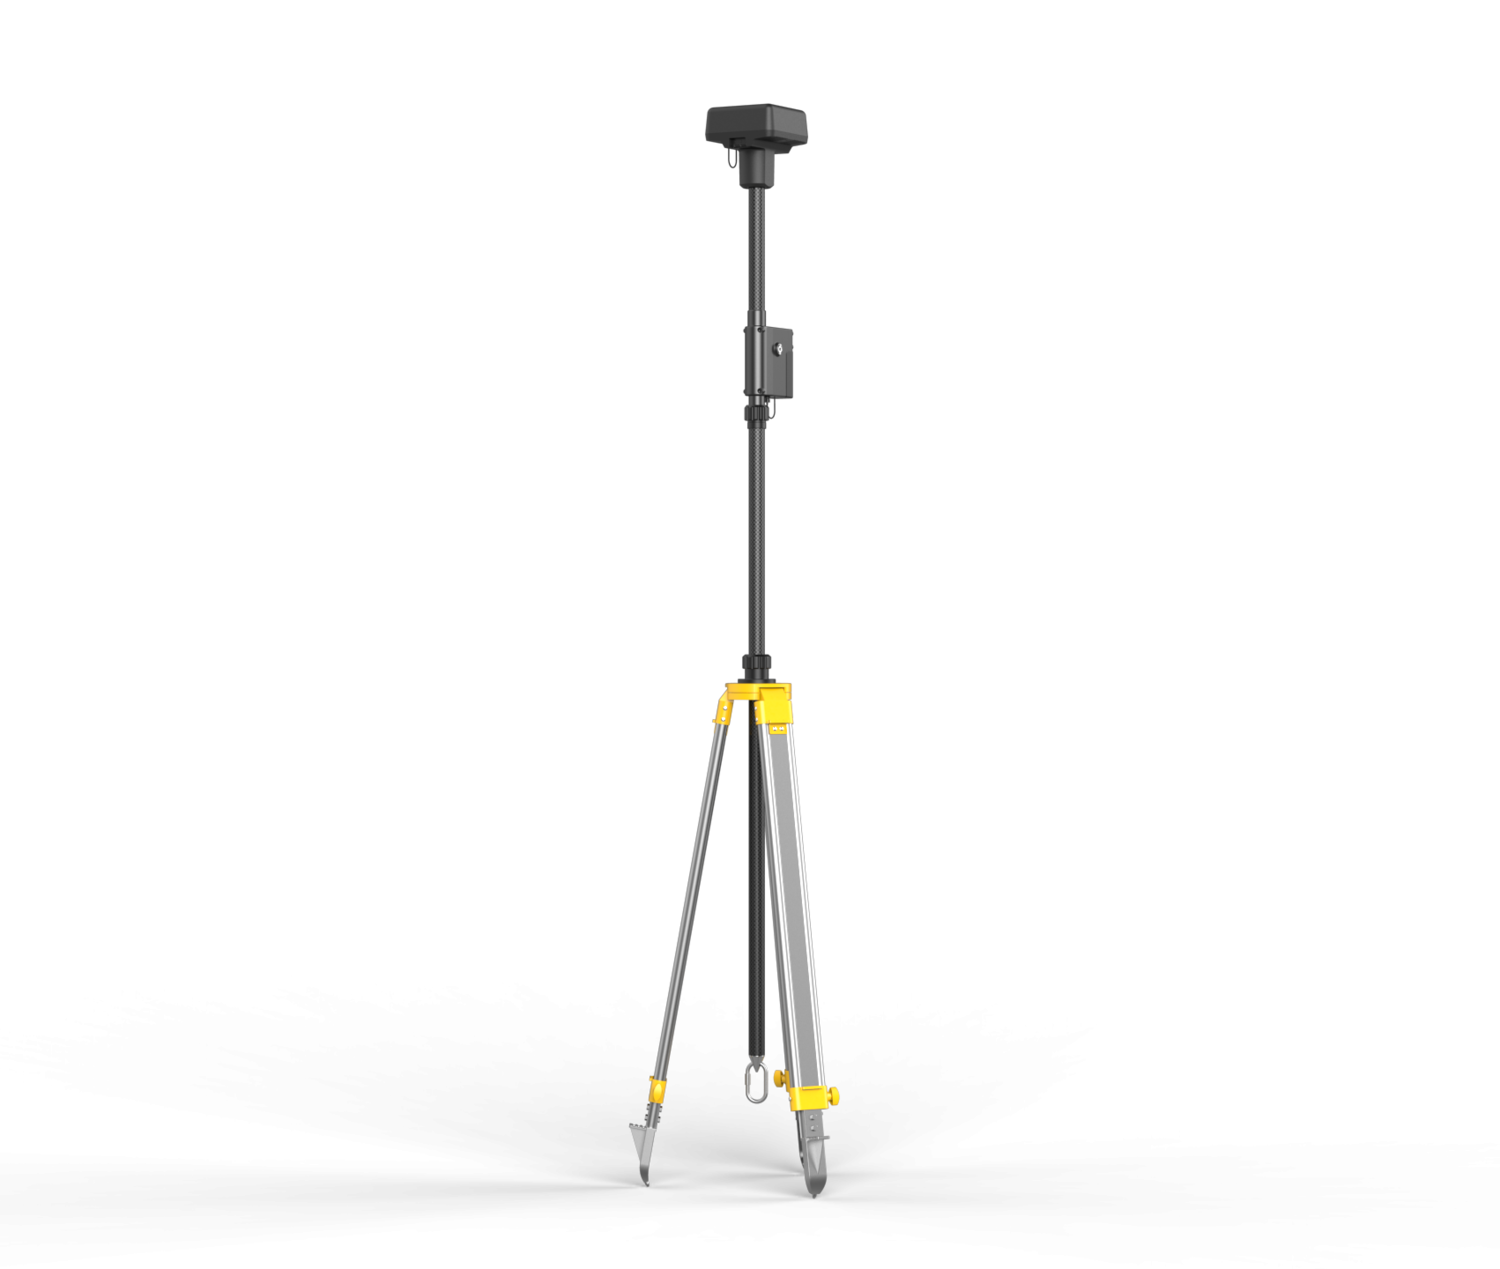
\includegraphics[height=1cm]{Chapters/Figures/base_stations/d-rtk-2.png} \\
    \midrule\addlinespace[1.5ex]
            Differentiator
            & 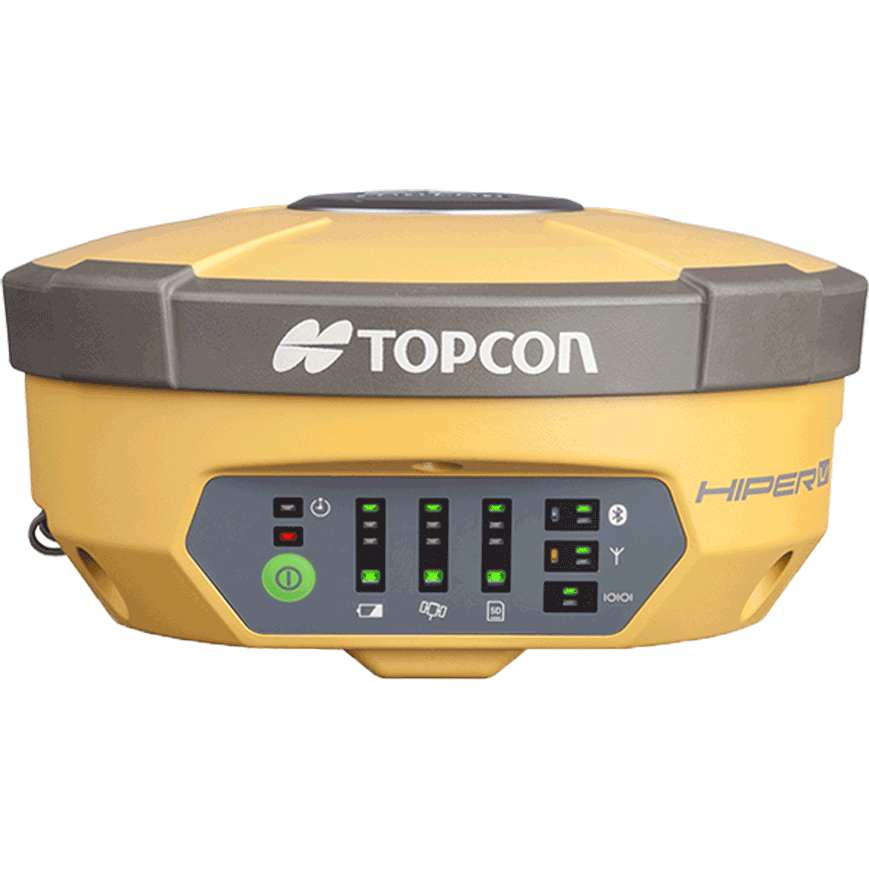
\includegraphics[height=1cm]{Chapters/Figures/base_stations/HiPer-V.png} \\
    \midrule\addlinespace[1.5ex]
            AC differentiator \\ with DC gain
            & 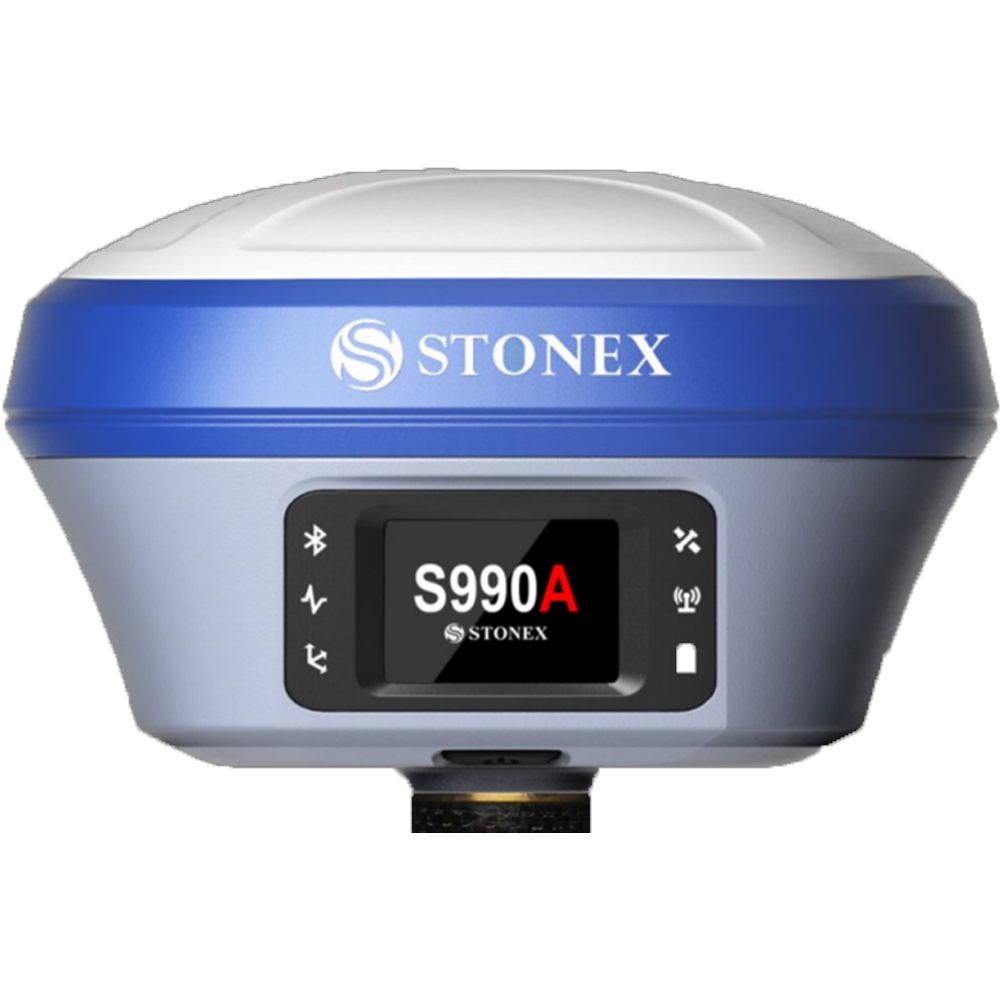
\includegraphics[height=1cm]{Chapters/Figures/base_stations/S990A.png} \\
    \bottomrule
        \end{tabular}
        \caption{A few basic circuit blocks and their frequency response for servo design.}
        \label{table4.2}
\end{table}
